\documentclass[11pt]{article}
% -------------------------------
% Shared packages and commands
% -------------------------------

% --- Page size & margins ---
\usepackage[a4paper,top=2cm,bottom=2.5cm,left=2cm,right=2cm]{geometry}

% --- Title formatting ---
\usepackage{titling}

% Move the whole title block up
\setlength{\droptitle}{-2em}

% Keep author and date on their own lines, just reduce the gaps
\pretitle{\begin{center}\LARGE\bfseries}%
\posttitle{\par\end{center}\vspace{-0.5em}} % space after title
\preauthor{\begin{center}\large}%
\postauthor{\par\end{center}\vspace{-0.5em}} % space after author
\predate{\begin{center}\small}%
\postdate{\par\end{center}\vspace{-1em}} % space after date block


% --- Math & theorem environments ---
\usepackage{amsmath, amssymb, amsthm}

% --- Graphics & tables ---
\usepackage{graphicx}
\usepackage{booktabs}

% --- Hyperlinks ---
\usepackage{hyperref}
\hypersetup{
  colorlinks=true,
  linkcolor=blue,
  urlcolor=blue
}

% --- Optional: underlined hyperlinks (remove if not desired) ---
% \usepackage[normalem]{ulem}
% \renewcommand\UrlFont{\uline}

% --- Custom macros (add your own below) ---
% \newcommand{\R}{\mathbb{R}}

\title{SPC707P Machine and Deep Learning — Week 01 Project}
\author{Kavit Tolia} 
\date{\today}

\usepackage{fancyhdr}
\usepackage{lastpage}

\begin{document}
\maketitle

\pagestyle{fancy}
\fancyhf{}%
\fancyfoot[C]{\thepage\ of \pageref{LastPage}}

% Make the 'plain' style (used on first page, after \maketitle, etc.) match:
\fancypagestyle{plain}{%
  \fancyhf{}%
  \fancyfoot[C]{\thepage\ of \pageref{LastPage}}
  \renewcommand{\headrulewidth}{0pt}
  \renewcommand{\footrulewidth}{0pt}
}

\section{Pick 5 of your favourite datasets}
I have picked the following 5 datasets for this week's project: \\
1. Adult Income or Census Income from US Census Bureau: \href{https://archive.ics.uci.edu/dataset/2/adult}{\underline{Adult Income}} \\
2. Air Quality or AirQualityUCI using sensors in Italy: \href{https://archive.ics.uci.edu/dataset/360/air+quality}{\underline{Air Quality}} \\
3. Micro Gas Turbine Electrical Energy Prediction: \href{https://archive.ics.uci.edu/dataset/994/micro+gas+turbine+electrical+energy+prediction}{\underline{Electrical Energy Prediction}} \\
4. Heart Disease (Cleveland): \href{https://archive.ics.uci.edu/dataset/45/heart+disease}{\underline{Heart Disease}} \\
5. Wine Quality (Red and White Vino Verde): \href{https://archive.ics.uci.edu/dataset/186/wine+quality}{\underline{Wine Quality}} 

\section{How many instances and features are in each dataset?}
\begin{table}[h!]
\centering
\begin{tabular}{lcc}
\hline
Dataset & Instances & Features \\
\hline
Adult Income & 32,561 (train only) & 14 \\
Air Quality & 9,258 & 15 \\
Electrical Energy & 71,225 & 1 \\
Heart Disease & 303 & 13 \\
Wine Quality & 1,599 (red) / 4,898 (white) & 11 \\
\hline
\end{tabular}
\caption{Basic properties of selected datasets.}
\end{table}

\section{What type of person might have collected this data?}
1. The adult income dataset would be collected by a \textbf{census bureau} \\
2. The air quality dataset would have been collected by a \textbf{government or environmental agency} \\
3. The electrical energy prediction dataset would have been collected by an \textbf{energy department} \\
4. The heart disease dataset would have been collected by a \textbf{medical institute} \\
5. The wine quality dataset would have been collected by a \textbf{wine producer}

\section{Why do I find each of the datasets interesting?}
1. Adult Income: It would be interesting to see how well demographics can predict income \\
2. Air Quality: I'm interested in understanding how certain attributes can determine extent of air pollution \\
3. Electrical Energy: I find time series analysis quite interesting, and this seemed quite realistic \\
4. Heart Disease: Understanding the effect of someone's attributes on heart disease can have very positive health impact \\
5. Wine Quality: \textbf{I love wine!}

\section{What are some deeper insights the datasets might reveal?}
1. Adult Income: If demographics can predict income, governments can guide policy to support their citizens \\
2. Air Quality: The data can be used to plan cities in a way which reduces air pollution without other changes \\
3. Electrical Energy: The data can show insights into how the turbine reacts to changes in control voltage \\
4. Heart Disease: If there is a link between certain factors and heart disease, we could have early prediction and reduce medical costs for individuals and governments \\
5. Wine Quality: A winemaker can derive an exact recipe to provide the highest quality wine

\section{What are some ethical or representative issues with the data?}
1. Adult Income: This data is from 1994 and may no longer represent the world today. While the features can help us with predicting income, it can be difficult to attribute rationale if there is a deeper layer of inherent socio-economic bias. \\
2. Air Quality: This is only from one location and might not be representative of other places across the globe. \\
3. Electrical Energy: The data might not generalise to other turbine types or environments. \\
4. Heart Disease: The data might not generalise to the broader demographic and could also lead to privacy issues given medical data. \\
5. Wine Quality: The ratings for each of the wine is subjective to an individual's preferences - it's difficult to remove human bias from the target variable.

\section{Data Cleansing}
For this task, I have decided to use the Adult Income dataset. I will attempt to fix any missing values and examine any other issues with the data. \\
I will explain the data issue, provide the code used to make any changes and highlight the fixed data. \\
- Once I loaded the data, I used \texttt{df.info()} to understand the data types of each of the features. \\
- For object types, I used \texttt{df[col].value\_counts} to understand missing data. \\
- For numerical types, I used \texttt{df.describe(include='all')} to understand missing data. \\
The dataset has '?' as a proxy for missing values. We can then use \texttt{df.replace} and \texttt{df.dropna} to delete rows with missing data. This removed 2,399 instances out of a total of 32,561. 

\begin{lstlisting}[caption={Cleaning Adult Income dataset}, label={lst:cleaning}]
import pandas as pd
import numpy as np
cols = ['age', 'workclass', 'fnlwgt', 'education', 'education_num', 'marital-status', 
        'occupation', 'relationship', 'race', 'sex', 'capital-gain', 'capital-loss', 
        'hours-per-week', 'native-country', 'income_class']
data_loc = '../data/raw/adult/adult.data'
df = pd.read_csv(data_loc, header=None, names=cols)
df.replace('?', np.nan, inplace=True)
df.dropna(inplace=True)
\end{lstlisting}

\section{Exploratory Data Analysis (EDA)}
I have also created a scatter matrix (on the following page) for a handful of numerical features. \\
The target is highlighted in a different colour (red for greater than 50K and blue for less than 50K). \\
We can make the following observations based on the scatter matrix: \\
- Higher levels of education are clearly linked to with a greater probability of earning more than 50K \\
- Very high capital gains also tend to appear only among higher income individuals (although these large gains are rare and the feature is very skewed with lots of zeros and a few hard-coded 99,999 values) \\
- Age doesn't seem to have a strong relationship with income \\
- There seems to be some trend between the number of hours worked and income, although this could be due to other factors \\

\vfill
\begin{center}
    \textit{Figure shown on next page $\rightarrow$}
\end{center}
\newpage

\newpage
\begin{figure}[h!]
  \centering
  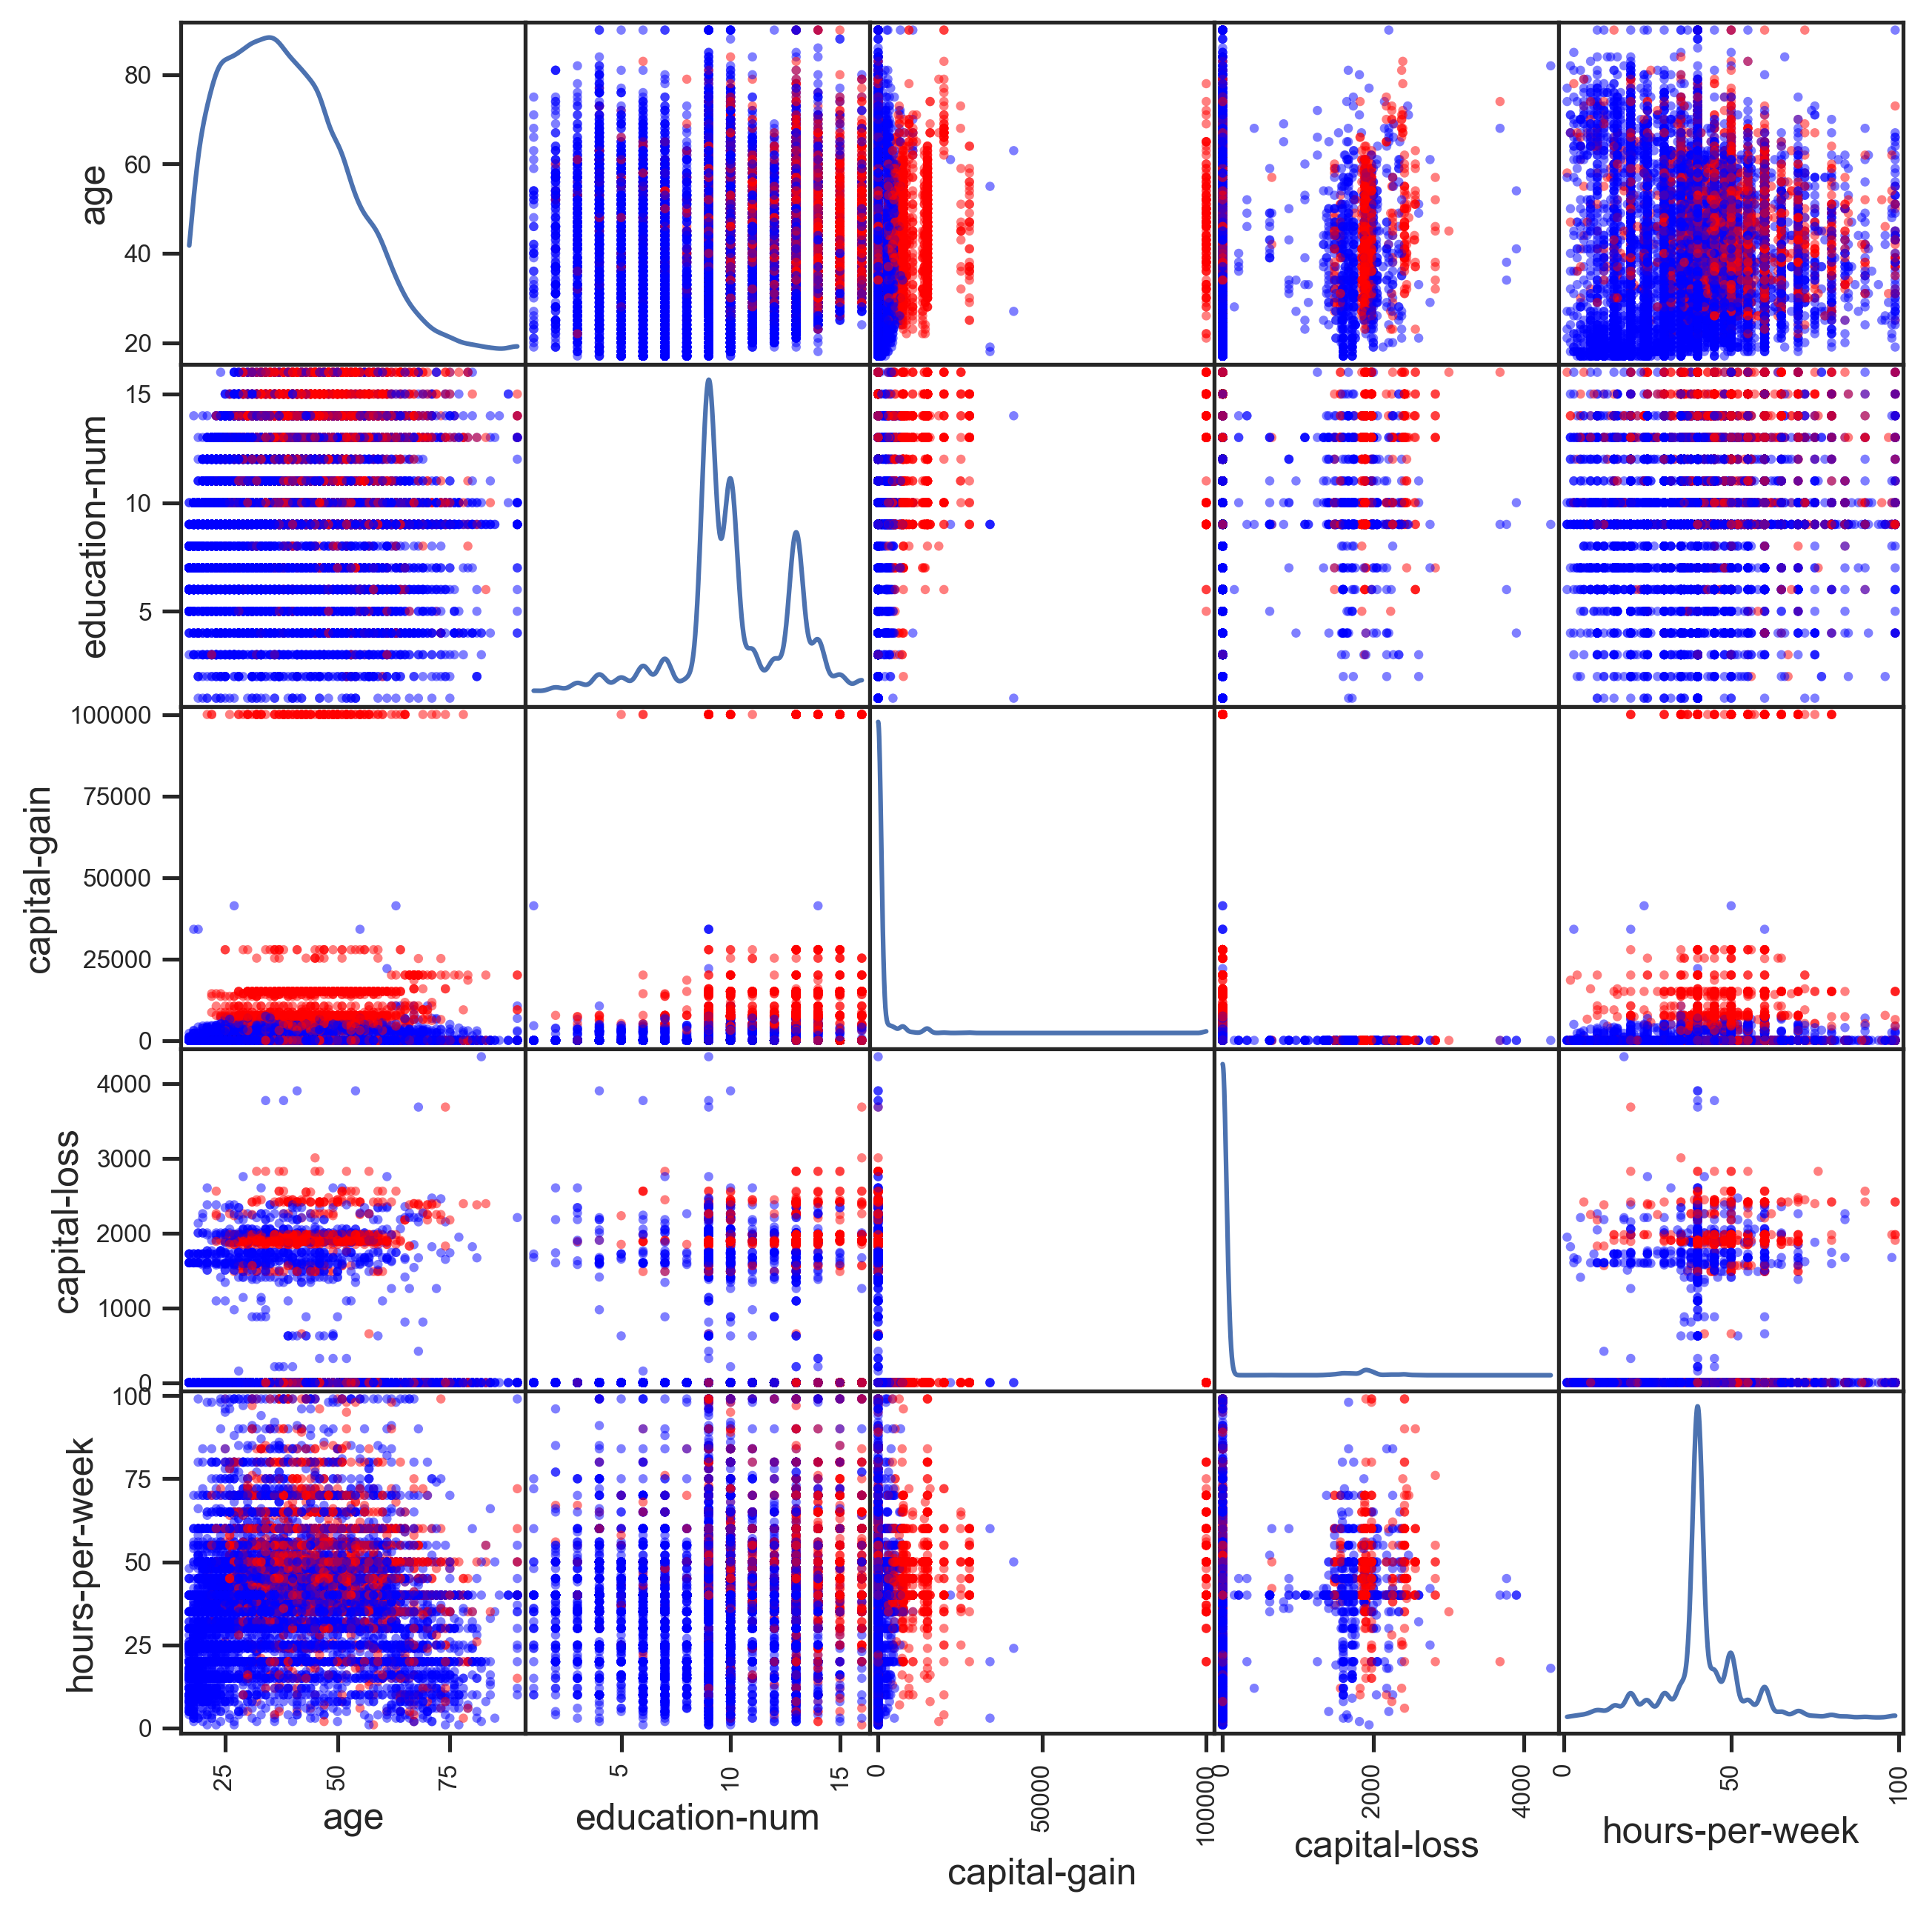
\includegraphics[width=\textwidth]{../scatter_matrix.png}
  \caption{Scatter matrix of selected continuous variables in the Adult Income dataset. \\
            The red dots highlight individuals with income higher than 50K and the blue dots for lower than 50K.}
  \label{fig:scatter}
\end{figure}

\end{document}
